\selectlanguage{english}

\section{Tree-level amplitudes}

\subsection{\texorpdfstring{$ e^+ e^- \rightarrow \mu^+ \mu^- $}{e+e- --> µ+µ-} scattering}

The $ e^+ e^- \rightarrow \mu^+ \mu^- $ scattering is the simplest process in QED and one of the most important in high-energy physics, as it is used to calibrate $ e^+ e^- $ colliders. \\
Recalling the Feynman rules for QED from \secref{sssec:qed-feyn}, the amplitude can be found from the only Feynman diagram of the process\footnotemark:
\begin{equation*}
  \begin{tikzpicture}[baseline=(r.base)]
    \begin{feynman}[inline=(r.base)]

      \vertex[dot] (a1) {};
      \vertex (l1) at ($(a1)+(-0.4,0)$) {\(e^-\)};

      \vertex[right=8cm of a1, dot] (a2) {};
      \vertex (l2) at ($(a2)+(+0.4,0)$) {\(\mu^-\)};

      \vertex[below=6em of a1, dot] (b1) {};
      \vertex (l3) at ($(b1)+(-0.4,0)$) {\(e^+\)};

      \vertex[below=6em of a2, dot] (b2) {};
      \vertex (l4) at ($(b2)+(+0.4,0)$) {\(\mu^+\)};

      \vertex[below=3em of a1] (c1) {};

      \vertex[right=2cm of c1, dot] (c2) {};

      \vertex[right=4cm of c2, dot] (c3) {};

      \vertex[below=1.1em of a1] (r);

      \diagram* {
        (a1) -- [fermion, momentum = \(p_1\)] (c2),
        (b1) -- [anti fermion, momentum' = \(p_2\)] (c2),

        (c3) -- [fermion, momentum = \(k_1\)] (a2),
        (c3) -- [anti fermion, momentum' = \(k_2\)] (b2),

        (c2) -- [photon, momentum = \(q\)] (c3),
      };
    \end{feynman}
  \end{tikzpicture}
\end{equation*}
with $ q = p_1 + p_2 = k_1 + k_2 $ by momentum conservation. By \eref{eq:mat-el}, then:
\begin{equation*}
  i \mathcal{M} = \bar{u}^{s_1}(k_1) (-i e \gamma^\mu) v^{s_2}(k_2) \frac{-i \eta_{\mu \nu}}{q^2 + i \epsilon} \bar{v}^{r_2}(p_2) (-i e \gamma^\nu) u^{r_1}(p_1) = \frac{i e^2}{q^2} \bar{u}^{s_1}(k_1) \gamma^\mu v^{s_2}(k_2) \bar{v}^{r_2}(p_2) \gamma_\mu u^{r_1}(p_1)
\end{equation*}

\footnotetext{Note that, if $ \ell \bar{\ell} \rightarrow \ell \bar{\ell} $, with $ \ell = e^-, \mu^- $, was considered instead, there would be a second Feynman diagram to computed:
\begin{equation*}
  \begin{tikzpicture}[baseline=(r.base)]
    \begin{feynman}[inline=(r.base)]

      \vertex[dot] (a1) {};
      \vertex (l1) at ($(a1)+(-0.4,0)$) {\(\ell\)};

      \vertex[right=8cm of a1, dot] (a2) {};
      \vertex (l2) at ($(a2)+(+0.4,0)$) {\(\bar{\ell}\)};

      \vertex[below=6em of a1, dot] (b1) {};
      \vertex (l3) at ($(b1)+(-0.4,0)$) {\(\ell\)};

      \vertex[below=6em of a2, dot] (b2) {};
      \vertex (l4) at ($(b2)+(+0.4,0)$) {\(\bar{\ell}\)};

      \vertex[below=3em of a1] (c1) {};

      \vertex[right=2cm of c1, dot] (c2) {};

      \vertex[right=4cm of c2, dot] (c3) {};

      \vertex[below=1.1em of a1] (r);

      \diagram* {
        (a1) -- [fermion, momentum = \(p_1\)] (c2),
        (c2) -- [fermion, momentum = \(k_1\)] (b1),

        (a2) -- [anti fermion, momentum' = \(p_2\)] (c3),
        (c3) -- [anti fermion, momentum' = \(k_2\)] (b2),

        (c2) -- [photon, momentum = \(q\)] (c3),
      };
    \end{feynman}
  \end{tikzpicture}
\end{equation*}
with $ q = p_1 - k_1 = k_2 - p_2 $.
}

\begin{lemma}[before upper = {\tcbtitle}]{Bi-spinor products}{}
  \begin{equation}
    (\bar{u} \gamma^\mu v)^* = \bar{v} \gamma^\mu u
  \end{equation}
\end{lemma}

\begin{proofbox}
  \begin{proof}
    $ (\bar{u} \gamma^\mu v)^* = v\dg (\gamma^\mu)\dg \bar{u}\dg = v\dg (\gamma^\mu)\dg (u\dg \gamma^0)\dg = v\dg (\gamma^\mu)\dg \gamma^0 u = v\dg \gamma^0 \gamma^\mu u = \bar{v} \gamma^\mu u $.
  \end{proof}
\end{proofbox}

With this lemma, it is easy to see that (as $ \bar{u} \gamma^\mu v \in \C $):
\begin{equation*}
  \begin{split}
    \abs{\mathcal{M}_{r_1,r_2,s_1,s_2}}^2
    & = \frac{e^4}{q^4} \bar{u}^{s_1}(k_1) \gamma^\mu v^{s_2}(k_2) \bar{v}^{r_2}(p_2) \gamma_\mu u^{r_1}(p_1) \bar{v}^{s_2}(k_2) \gamma^\nu u^{s_1}(k_1) \bar{u}^{r_1}(p_1) \gamma_\nu v^{r_2}(p_2) \\
    & = \frac{e^4}{q^4} \bar{u}^{s_1}(k_1) \gamma^\mu v^{s_2}(k_2) \bar{v}^{s_2}(k_2) \gamma^\nu u^{s_1}(k_1) \bar{v}^{r_2}(p_2) \gamma_\mu u^{r_1}(p_1) \bar{u}^{r_1}(p_1) \gamma_\nu v^{r_2}(p_2)
  \end{split}
\end{equation*}
This matrix element has explicit dependence on spin states: although not impossible, it is difficult to experimentally retain control over them, both in the initial- and final-state. For this reason, it is convenient to consider a matrix element which is averaged over initial spin states and summed over final spin states (as usually the detector does not distinguish them):
\begin{equation}
  \abs{\mathcal{M}}^2 = \frac{1}{2} \sum_{r_1 = 1,2} \frac{1}{2} \sum_{r_2 = 1,2} \sum_{s_1} \sum_{s_2 = 1,2} \abs{\mathcal{M}_{r_1,r_2,s_1,s_2}}^2
\end{equation}
Recalling \eref{eq:spinor-sums} and writing spinor indices explicitly, the first half of the matrix element is:
\begin{multline*}
  \frac{e^4}{4q^4} \sum_{s_1,s_2 = 1,2} \sum_{a,b,c,d = 1}^{4} [\bar{u}^{s_1}(k_1)]_a \gamma^\mu_{ab} [v^{s_2}(k_2)]_b [\bar{v}^{s_2}(k_2)]_c \gamma^\nu_{cd} [u^{s_1}(k_1)]_d \\
  = \frac{e^4}{4q^4} \sum_{s_1,s_2 = 1,2} \sum_{a,b,c,d = 1}^{4} [\slashed{k}_1 + m_\mu]_{da} \gamma^\mu_{ab} [\slashed{k}_2 - m_\mu]_{bc} \gamma^\nu_{cd} = \frac{e^4}{4q^4} \sum_{s_1,s_2 = 1,2} \tr\{(\slashed{k}_1 + m_\mu) \gamma^\mu (\slashed{k}_2 - m_\mu) \gamma^\nu\}
\end{multline*}
The unpolarized matrix element then is:
\begin{equation}
  \abs{\mathcal{M}}^2 = \frac{e^4}{4q^4} \sum_{r_1,r_2,s_1,s_2 = 1,2} \tr\{(\slashed{k}_1 + m_\mu) \gamma^\mu (\slashed{k}_2 - m_\mu) \gamma^\nu\} \tr\{(\slashed{p}_1 + m_e) \gamma_\mu (\slashed{p}_2 - m_e) \gamma_\nu\}
  \label{eq:unp-mat-el-pre}
\end{equation}
This approach is general: any QED amplitude involving external fermions can be simplified into traces of products of gamma matrices, when squared and summed/averaged over spin states, hence eliminating explicit dependence on spinors.

\subsubsection{Traces}

Due to their importance in QED, traces of gamma matrices should be studied systematically.

\begin{proposition}{Odd number of gamma matrices}{odd-gamma}
  For any $ n \in \N $ odd:
  \begin{equation}
    \tr\{\gamma^{\mu_1} \dots \gamma^{\mu_n}\} = 0
  \end{equation}
\end{proposition}

\begin{proofbox}
  \begin{proof}
    As $ \{\gamma^\mu , \gamma^5\} = 0 $ and given the cyclic property of the trace:
    \begin{equation*}
      \begin{split}
        \tr\{\gamma^{\mu_1} \dots \gamma^{\mu_n}\}
        & = \tr\{\gamma^5 \gamma^5 \gamma^{\mu_1} \dots \gamma^{\mu_n}\} = - \tr\{\gamma^5 \gamma^{\mu_1} \gamma^5 \dots \gamma^{\mu_n}\} \\
        & = (-1)^n \tr\{\gamma^5 \gamma^{\mu_1} \dots \gamma^{\mu_n} \gamma^5\} = (-1)^n \tr\{\gamma^5 \gamma^5 \gamma^{\mu_1} \dots \gamma^{\mu_n}\} = (-1)^n \tr\{\gamma^{\mu_1} \dots \gamma^{\mu_n}\}
      \end{split}
    \end{equation*}
    Therefore, the trace vanishes for any odd $ n \in \N $.
  \end{proof}
\end{proofbox}

\begin{proposition}[before upper = {\tcbtitle}]{Even number of gamma matrices}{}
  \begin{equation}
    \tr\{\gamma^\mu \gamma^\nu\} = 4 \eta^{\mu \nu}
  \end{equation}
  \begin{equation}
    \tr\{\gamma^\mu \gamma^\nu \gamma^\rho \gamma^\sigma\} = 4 \left( \eta^{\mu \nu} \eta^{\rho \sigma} - \eta^{\mu \rho} \eta^{\nu \sigma} + \eta^{\mu \sigma} \eta^{\nu \rho} \right)
  \end{equation}
\end{proposition}

\begin{proofbox}
  \begin{proof}
    Using $ \{\gamma^\mu , \gamma^\nu\} = 2 \eta^{\mu \nu} \tens{I}_4 $:
    \begin{equation*}
      \tr\{\gamma^\mu \gamma^\nu\} = \tr\{ 2\eta^{\mu \nu} \tens{I}_4 - \gamma^\nu \gamma^\mu\} = 8 \eta^{\mu \nu} - \tr\{\gamma^\mu \gamma^\nu\}
    \end{equation*}
    \begin{equation*}
      \begin{split}
        \tr\{\gamma^\mu \gamma^\nu \gamma^\rho \gamma^\sigma\}
        & = \tr\{2\eta^{\mu \nu} \gamma^\rho \gamma^\sigma - \gamma^\nu \gamma^\mu \gamma^\rho \gamma^\sigma\} \\
        & = \tr\{2\eta^{\mu \nu} \gamma^\rho \gamma^\sigma - \gamma^\nu 2 \eta^{\mu \rho} \gamma^\sigma + \gamma^\nu \gamma^\rho 2 \eta^{\mu \sigma} - \gamma^\nu \gamma^\rho \gamma^\sigma \gamma^\mu\} \\
        & = 4 \left( \eta^{\mu \nu} \eta^{\rho \sigma} - \eta^{\mu \rho} \eta^{\nu \sigma} + \eta^{\mu \sigma} \eta^{\nu \rho} \right) - \tr\{\gamma^\mu \gamma^\nu \gamma^\rho \gamma^\sigma\}
      \end{split}
    \end{equation*}
  \end{proof}
\end{proofbox}

In general, the trace of the product of $ n $ gamma matrices can be reduced to traces of products of $ n-2 $ gamma matrices. Traces involving $ \gamma^5 \defeq i \gamma^0 \gamma^1 \gamma^2 \gamma^3 $ are of interest too.

\begin{proposition}{Odd number of gamma matrices}{}
  For any $ n \in \N $ odd:
  \begin{equation}
    \tr\{\gamma^{\mu_1} \dots \gamma^{\mu_n} \gamma^5\} = 0
  \end{equation}
\end{proposition}

\begin{proofbox}
  \begin{proof}
    As in the proof of \pref{prop:odd-gamma}:
    \begin{equation*}
      \tr\{\gamma^{\mu_1} \dots \gamma^{\mu_n} \gamma^5\} = (-1)^n \tr\{\gamma^5 \gamma^{\mu_1} \dots \gamma^{\mu_n} \gamma^5 \gamma^5\} = (-1)^n \tr\{\gamma^{\mu_1} \dots \gamma^{\mu_n} \gamma^5\}
    \end{equation*}
    which vanishes for any odd $ n \in \N $.
  \end{proof}
\end{proofbox}

\begin{proposition}[before upper = {\tcbtitle}]{Even number of gamma matrices}{}
  \begin{equation}
    \tr \gamma^5 = \tr\{\gamma^\mu \gamma^\nu \gamma^5\} = 0
  \end{equation}
  \begin{equation}
    \tr\{\gamma^\mu \gamma^\nu \gamma^\rho \gamma^\sigma \gamma^5\} = -4i \epsilon^{\mu \nu \rho \sigma}
  \end{equation}
\end{proposition}

\begin{proofbox}
  \begin{proof}
    Recalling that $ \{\gamma^5 , \gamma^\mu\} = 0 $:
    \begin{equation*}
      \tr \gamma^5 = \tr\{\gamma^0 \gamma^0 \gamma^5\} = - \tr\{\gamma^0 \gamma^5 \gamma^0\} = - \tr\{\gamma^0 \gamma^0 \gamma^5\} = - \tr \gamma^5
    \end{equation*}
    Analogously, given $ \alpha \neq \mu , \nu $ (so that $ \{\gamma^\mu , \gamma^\alpha\} = \{\gamma^\nu , \gamma^\alpha\} = \{\gamma^5 , \gamma^\alpha\} = 0 $):
    \begin{equation*}
      \tr\{\gamma^\mu \gamma^\nu \gamma^5\} = \tr\{\gamma^0 \gamma^0 \gamma^\mu \gamma^\nu \gamma^5\} = (-1)^3 \tr\{\gamma^0 \gamma^\mu \gamma^\nu \gamma^5 \gamma^0\} = - \tr\{\gamma^\mu \gamma^\nu \gamma^5\}
    \end{equation*}
    Consider now $ \tr\{\gamma^\mu \gamma^\nu \gamma^\rho \gamma^\sigma \gamma^5\} $: the above reasoning still applies if any couple of equal indices is present, therefore the trace must be proportional to $ \epsilon^{\mu \nu \rho \sigma} $, which agrees with the anti-commutation relation of different gamma matrices. Computing $ \tr\{\gamma^0 \gamma^1 \gamma^2 \gamma^3 \gamma^5\} $ gives the correct proportionality constant $ -4i $.
  \end{proof}
\end{proofbox}

It is useful to recall an identity for the Levi-Civita symbol.

\begin{lemma}{Levi-Civita symbol}{}
  Given $ n \in \N $ and $ \{i_k\}_{k = 1,\dots,n} , \{j_k\}_{k = 1,\dots,n} \subset \{1,\dots,n\} $, then:
  \begin{equation}
    \epsilon_{i_1 \dots i_k i_{k+1} \dots i_n} \epsilon^{i_1 \dots i_k j_{k+1} \dots j_n} = n! \delta^{j_{k+1} \dots j_n}_{i_{k+1} i_n}
  \end{equation}
  where the \bclemma{generalized Kronecker delta} is defined as:
  \begin{equation}
    \delta^{\mu_1 \dots \mu_p}_{\nu_1 \dots \nu_p} \defeq
    \begin{vmatrix}
      \delta^{\mu_1}_{\nu_1} & \dots & \delta^{\mu_p}_{\nu_1} \\
      \vdots & \ddots & \vdots \\
      \delta^{\mu_1}_{\nu_p} & \dots & \delta^{\mu_p}_{\nu_p}
    \end{vmatrix}
  \end{equation}
\end{lemma}

Gamma matrices' contractions are important too.

\begin{proposition}[before upper = {\tcbtitle}]{Contractions}{}
  \begin{equation}
    \gamma^\mu \gamma_\mu = 4
  \end{equation}
  \begin{equation}
    \gamma^\mu \gamma^\nu \gamma_\mu = -2 \gamma^\nu
  \end{equation}
  \begin{equation}
    \gamma^\mu \gamma^\nu \gamma^\rho \gamma_\mu = 4 \eta^{\nu \rho}
  \end{equation}
  \begin{equation}
    \gamma^\mu \gamma^\nu \gamma^\rho \gamma^\sigma \gamma_\mu = -2 \gamma^\nu \gamma^\rho \gamma^\sigma
  \end{equation}
\end{proposition}

\subsubsection{Unpolarized matrix element}

It is now possible to evaluate the matrix element in \eref{eq:unp-mat-el-pre}. Explicitly, the traces are:
\begin{equation*}
  \begin{split}
    \tr\{(\slashed{k}_1 + m_\mu) \gamma^\mu (\slashed{k}_2 - m_\mu) \gamma^\nu\}
    & = \tr\{{k_1}_\alpha {k_2}_\beta \gamma^\alpha \gamma^\mu \gamma^\beta \gamma^\nu + m_\mu {k_2}_\beta \gamma^\mu \gamma^\beta \gamma^\nu - {k_1}_\alpha m_\mu \gamma^\alpha \gamma^\mu \gamma^\nu - m_\mu^2 \gamma^\mu \gamma^\nu\} \\
    & = {k_1}_\alpha {k_2}_\beta 4 \left( \eta^{\alpha \mu} \eta^{\beta \nu} - \eta^{\alpha \beta} \eta^{\mu \nu} + \eta^{\alpha \nu} \eta^{\mu \beta} \right) - m_\mu^2 4 \eta^{\mu \nu} \\
    & = 4 \left[ {k_1}^\mu {k_2}^\nu + {k_1}^\nu {k_2}^\mu - \eta^{\mu \nu} \left( k_1 \cdot k_2 + m_\mu^2 \right) \right]
  \end{split}
\end{equation*}
where $ u \cdot v \equiv u^\mu v_\mu $. The other trace is analogous, so that:
\begin{equation*}
  \begin{split}
    \abs{\mathcal{M}}^2
    = \frac{4e^4}{q^4} & \big[ {k_1}^\mu {k_2}^\nu + {k_1}^\nu {k_2}^\mu - \eta^{\mu \nu} \left( k_1 \cdot k_2 + m_\mu^2 \right) \big] \big[ {p_1}_\mu {p_2}_\mu + {p_1}_\nu {p_2}_\mu - \eta_{\mu \nu} \left( p_1 \cdot p_2 + m_e^2 \right) \big] \\
    = \frac{4e^4}{q^4} & \big[ (k_1 \cdot p_1) (k_2 \cdot p_2) + (k_1 \cdot p_2) (k_2 \cdot p_1) - (p_1 \cdot p_2) (k_1 \cdot k_2) - m_\mu^2 (p_1 \cdot p_2) + \\
    & (k_1 \cdot p_2) (k_2 \cdot p_1) + (k_1 \cdot p_1) (k_2 \cdot p_2) - (p_1 \cdot p_2) (k_1 \cdot k_2) - m_\mu^2 (p_1 \cdot p_2) + \\
    & - 2 (k_1 \cdot k_2) (p_1 \cdot p_2) - 2 m_e^2 (k_1 \cdot k_2) + \\
    & + 4 (k_1 \cdot k_2) (p_1 \cdot p_2) + 4 m_e^2 (k_1 \cdot k_2) + 4 m_\mu^2 (p_1 \cdot p_2) + 4 m_\mu^2 m_e^2 \big] \\
    = \frac{8e^4}{q^4} & \big[ (k_1 \cdot p_1) (k_2 \cdot p_2) + (k_1 \cdot p_2) (k_2 \cdot p_1) + m_\mu^2 (p_1 \cdot p_2) + m_e^2 (k_1 \cdot k_2) + 2 m_\mu^2 m_e^2 \big] \\
  \end{split}
\end{equation*}
As $ m_e \sim 10^{-4} m_\mu $, it is possible to neglect terms which contain $ m_e $, thus the unpolarized matrix element is:
\begin{equation}
  \abs{\mathcal{M}}^2 = \frac{8e^4}{q^4} \left[ (k_1 \cdot p_1) (k_2 \cdot p_2) + (k_1 \cdot p_2) (k_2 \cdot p_1) + m_\mu^2 (p_1 \cdot p_2) \right]
\end{equation}
Note that, for a generic $ 2 \rightarrow 2 $ process, the unpolarized matrix element depends on 4 momenta, i.e. 16 variables. However, momentum conservation reduces this number by 4, as $ k_1 + k_2 = p_1 + p_2 $ (4 equations), and mass-shell conditions on these 4 momenta reduces it further by 4. This leaves only 8 variables, but 6 of them are fixed by Lorentz invariance\footnotemark (from 6 independent generators of $ \lorg $): the unpolarized matrix element hence only depends on 2 independent variables.

\footnotetext{Note that momentum conservation is a consequence of traslational invariance, therefore it can be united to Lorentz invariance to get Poincaré invariance, and indeed $ \pog $ has $ 6 + 4 = 10 $ independent generators.}

\begin{definition}{Mandelstam variables}{}
  Given a $ 2 \rightarrow 2 $ scattering such that $ i_1(k_1) + i_2(k_2) \rightarrow f_1(p_1) + f_2(p_2) $, then the \bcdef{Mandelstam variables} are defined as:
  \begin{equation}
    s \defeq (p_1 + p_2)^2 = (k_1 + k_2)^2
  \end{equation}
  \begin{equation}
    t \defeq (k_1 - p_1)^2 = (k_1 - p_2)^2
  \end{equation}
  \begin{equation}
    u \defeq (k_1 - p_2)^2 = (k_2 - p_1)^2
  \end{equation}
\end{definition}

\begin{proposition}{}{}
  Only two Mandelstam variables are independent, as:
  \begin{equation}
    s + t + u = m_{i_1}^2 + m_{i_2}^2 + m_{f_1}^2 + m_{f_2}^2
  \end{equation}
\end{proposition}

\begin{proofbox}
  \begin{proof}
    By direct calculation, using momentum conservation:
    \begin{equation*}
      \begin{split}
        s + t + u
        & = p_1^2 + p_2^2 + 2 p_1 \cdot p_2 + k_1^2 + p_1^2 - 2 k_1 \cdot p_1 + k_2^2 + p_1^2 - 2 k_2 \cdot p_1 \\
        & = 3p_1^2 + p_2^2 + k_1^2 + k_2^2 - 2p_1 \cdot (k_1 + k_2 - p_2) = p_1^2 + p_2^2 + k_1^2 + k_2^2
      \end{split}
    \end{equation*}
    Mass-shell conditions yield the thesis.
  \end{proof}
\end{proofbox}

It is possible to parametrize the 2 degrees of freedom of $ e^+e^- \rightarrow \mu^+\mu^- $ scattering with two Mandelstam variables, which for this process can be expressed as:
\begin{equation*}
  s = 2 (k_1 \cdot k_2 + m_\mu^2) = 2 (p_1 \cdot p_2 + m_e^2)
\end{equation*}
\begin{equation*}
  t = -2 k_1 \cdot p_1 + m_e^2 + m_\mu^2 = -2 k_2 \cdot p_2 + m_e^2 + m_\mu^2
\end{equation*}
\begin{equation*}
  u = -2 k_2 \cdot p_1 + m_e^2 + m_\mu^2 = -2 k_1 \cdot p_2 + m_e^2 + m_\mu^2
\end{equation*}
Neglecting terms with $ m_e $, it is possible to write:
\begin{equation*}
  \abs{\mathcal{M}}^2 = \frac{8e^4}{s^2} \left[ \frac{t - m_\mu^2}{2} \frac{t - m_\mu^2}{2} + \frac{u - m_\mu^2}{2} \frac{u - m_\mu^2}{2} + m_\mu^2 \frac{s}{2} \right]
\end{equation*}
which is:
\begin{equation}
  \abs{\mathcal{M}}^2 = \frac{2e^4}{s^2} \left[ (t - m_\mu)^2 + (u - m_\mu)^2 + 2m_\mu^2 s \right]
  \label{eq:mat-el-mand}
\end{equation}
To compare this theoretical prediction with experimental data, however, it is better to choose an energy and an angle as the 2 independent variables. To do so, it is necessary to choose a reference frame: a natural choise is the \bctxt{center-of-mass frame}, defined as the frame in which $ \ve{p}_1 = - \ve{p}_2 $. In this RF, momenta are parametrized as (see Fig. \ref{com-rf}):
\begin{equation*}
  p_1 = (E, E \hat{\ve{e}}_z) \qquad p_2 = (E, -E \hat{\ve{e}}_z) \qquad k_1 = (E, \ve{k}) \qquad k_2 = (E, -\ve{k})
\end{equation*}
with:
\begin{equation*}
  \abs{\ve{k}} = \sqrt{E^2 - m_\mu^2} \qquad \ve{k} \cdot \hat{\ve{e}}_z = \abs{\ve{k}} \cos \theta
\end{equation*}

\begin{figure}
  \centering
  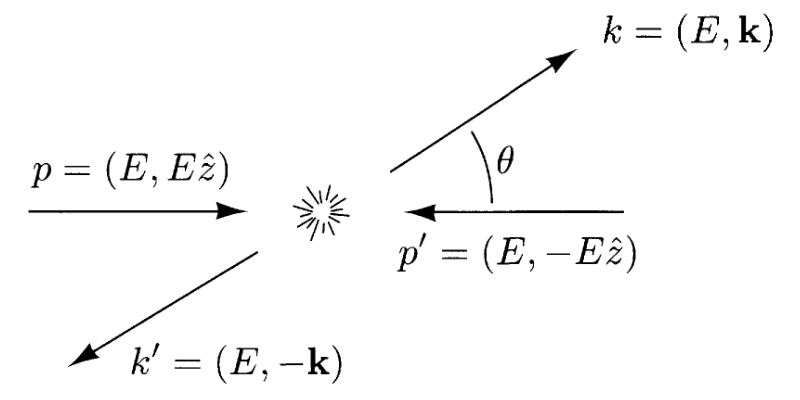
\includegraphics[width = 0.50 \textwidth]{imgs/com-rf.png}
  \caption{Center-of-mass RF for a $ 2 \rightarrow 2 $ scattering process.}
  \label{com-rf}
\end{figure}

Note that this is the most genera expression for $ 2 \rightarrow 2 $ scattering with $ m_{i_1} = m_{i_2} $ and $ m_{f_1} = m_{f_2} $. In this frame, the Mandelstam variables are:
\begin{equation*}
  s = 4E^2 \equiv E_\text{cm}^2
\end{equation*}
\begin{equation*}
  t = -2 (E^2 - E \abs{\ve{k}} \cos \theta) + m_e^2 + m_\mu^2 \approx -2E (E - \abs{\ve{k}} \cos \theta) + m_\mu^2
\end{equation*}
\begin{equation*}
  u = -2 (E^2 + E \abs{\ve{k}} \cos \theta) + m_e^2 + m_\mu^2 \approx -2E (E - \abs{\ve{k}} \cos \theta) + m_\mu^2
\end{equation*}
Inserting into \eref{eq:mat-el-mand}:
\begin{equation*}
  \begin{split}
    \abs{\mathcal{M}}^2
    & = \frac{2e^4}{16 E^4} \left[ 4E^2 (E - \abs{\ve{k}} \cos \theta)^2 + 4E^2 (E - \abs{\ve{k}} \cos \theta)^2 + 8 m_\mu^2 E^2 \right] \\
    & = \frac{e^4}{2E^2} \left[ (E - \abs{\ve{k}} \cos \theta)^2 + (E - \abs{\ve{k}} \cos \theta)^2 + 2m_\mu^2 \right] \\
    & = e^4 \left[ 1 + \frac{\abs{\ve{k}}^2}{E^2} \cos^2 \theta + \frac{m_\mu^2}{E^2} \right] = \left[ 1 + \frac{m_\mu^2}{E^2} + \left( 1 - \frac{m_\mu^2}{E^2} \right) \cos^2 \theta \right]
  \end{split}
\end{equation*}

\subsubsection{Unpolarized cross-section}

In general, the \bctxt{cross-section} generalizes the geometric section of an object in the context of scattering processes.










